 \providecommand{\main}{../../..}
\documentclass[\main/main.tex]{subfiles}
\begin{document}
\section{Caratterizzazione dei lati che appartengono ad alberi ricoprenti di costo minimo}

\begin{minipage}{\textwidth}
  \begin{minipage}{.83\textwidth}
    \flushleft
    \begin{theorem}[Caratterizzazione dei lati che appartengono ad alberi ricoprenti di costo minimo]
      Sia $G_{T^*} = (\mathcal{V}, T^*)$ un albero di costo minimo. Per un qualunque $l \in E$ si ha che $l \in T^*$ se e solo se esiste un $S \subset \mathcal{V}$ tale che $l = \argmin\crl{c_f: f \in \delta(S)}$, dove $\delta(S)$ è un taglio, cioè un insieme di lati che hanno un vertice in $S$ ed un vertice in $\mathcal{V} \bs S$.
    \end{theorem}
  \end{minipage}\hfill
  \begin{minipage}{0.15\textwidth}\center
    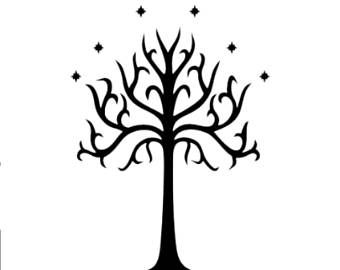
\includegraphics[width=\textwidth]{random/tree}
  \end{minipage}
\end{minipage}

\begin{proof}
  Per assurdo sia $l \not\in T^*$. Allora $T^* \cup \crl{l}$ contiene un ciclo $C(T^*, l)$. Sia $f \in C(T^*, l) \cap \delta(S) \Rightarrow T^* \cup \crl{l} \bs \crl{f}$ è albero ricoprende. Essendo $T^*$ minimo e $l = \argmin{c_f}$, allora $c_l \leq c_f$, da cui l'assurdo.
\end{proof}

\begin{proof}
  Dato $l \in T^*$, sia $S$ uno degli insiemi di nodi di una delle componenti connesse in $G' = \rnd{\mathcal{N}, T \bs \crl{l}}$. Per assurdo $\exists f \in \delta\rnd{S}\bs \crl{l}$ con $c_f < c_l$. Allora $T^*\cup \crl{f} \bs \crl{l}$ costa meno di $T^*$, da cui l'assurdo.
\end{proof}

\end{document}